\documentclass[12pt, a4paper]{article}
\setlength{\oddsidemargin}{0.5cm}
\setlength{\evensidemargin}{0.5cm}
\setlength{\topmargin}{-1.6cm} 
\setlength{\leftmargin}{0.5cm} 
\setlength{\rightmargin}{0.5cm} 
\setlength{\textheight}{24.00cm} 
\setlength{\textwidth}{15.00cm} 

%\parindent 2pt
%\parskip 5pt
\usepackage[utf8]{inputenc}
%\usepackage{glossaries}
\usepackage[acronym]{glossaries}
\usepackage{xcolor}
\usepackage{graphicx}
\usepackage{datetime}
\usepackage{courier}
\usepackage{array}

\title{Machine Learning in Terpenes' Classification}
\date{February 28, 2020}
\author{Deepkumar Shah \\Jodrey School of Computer Science \\Acadia University, Wolfville, NS, Canada, B4P 2R6 \\[1 cm]{\small Thesis Supervisor: Daniel L. Silver} \\{\small Co-supervisor: Andrew McIntyre}}

%   Generate the environment for the abstract:
\newcommand\summaryname{Abstract}
\newenvironment{Abstract}%
    {\small\begin{center}%
    \bfseries{\summaryname} \end{center}}

\makeglossaries

\newglossaryentry{rel abund}
{
    name=relative abundance,
    description={Amount of an ion produced in comparison to the most abundant ion.}
}

\newglossaryentry{PCA}
{
    name=Principal Component Analysis,
    description={A statistical method that describes the data by inter-correlated dependant variables}
}

%\title{How to create a glossary}
%\author{ }
%\date{ }

\setlength{\parindent}{4em}
\setlength{\parskip}{1em}
\renewcommand{\baselinestretch}{1.25}
 
\begin{document}
\pagenumbering{gobble}
\maketitle

%\newpage
\pagenumbering{arabic}

\begin{Abstract}
Traditionally, separation and classification of terpenes from food samples is done with the help of two processes, namely: Gas Chromatography (GC) (separate terpenes from each other) and Mass Spectrometry (MS) (detects the separated terpenes) \cite{de2000} \cite{Jiang2016}. A mass spectrum, generated by mass spectrometry is matched by a chemist from a existing database of mass spectra of various samples. Artificial Neural Networks (ANNs), Support Vector Machines (SVMs) and Deep Learning, in particular, have been widely adopted for many modern supervised learning tasks (e.g., classification and regression problems) and are known for their state-of-the-art generalization performance. The proposed research uses ANNs as part of a tool that can read mass spectra and automatically detect the presence of various terpenes and determine their relative proportions. Early classification results using the SVM algorithm returns an accuracy of 91.43\% for four terpenes.

\end{Abstract}

\newpage

\section{Introduction}
\subsection{Synopsis}
Terpenes are an important class of organic compounds that are present in foods that we consume every day. For instance, myrcene is found in mango, humulene in coriander. Some commonly used terpenes consumed in our day-to-day life are shown in fig. \ref{fig:baseterpenes}. \begin{figure}[!ht]
\centering
    \begin{center}
        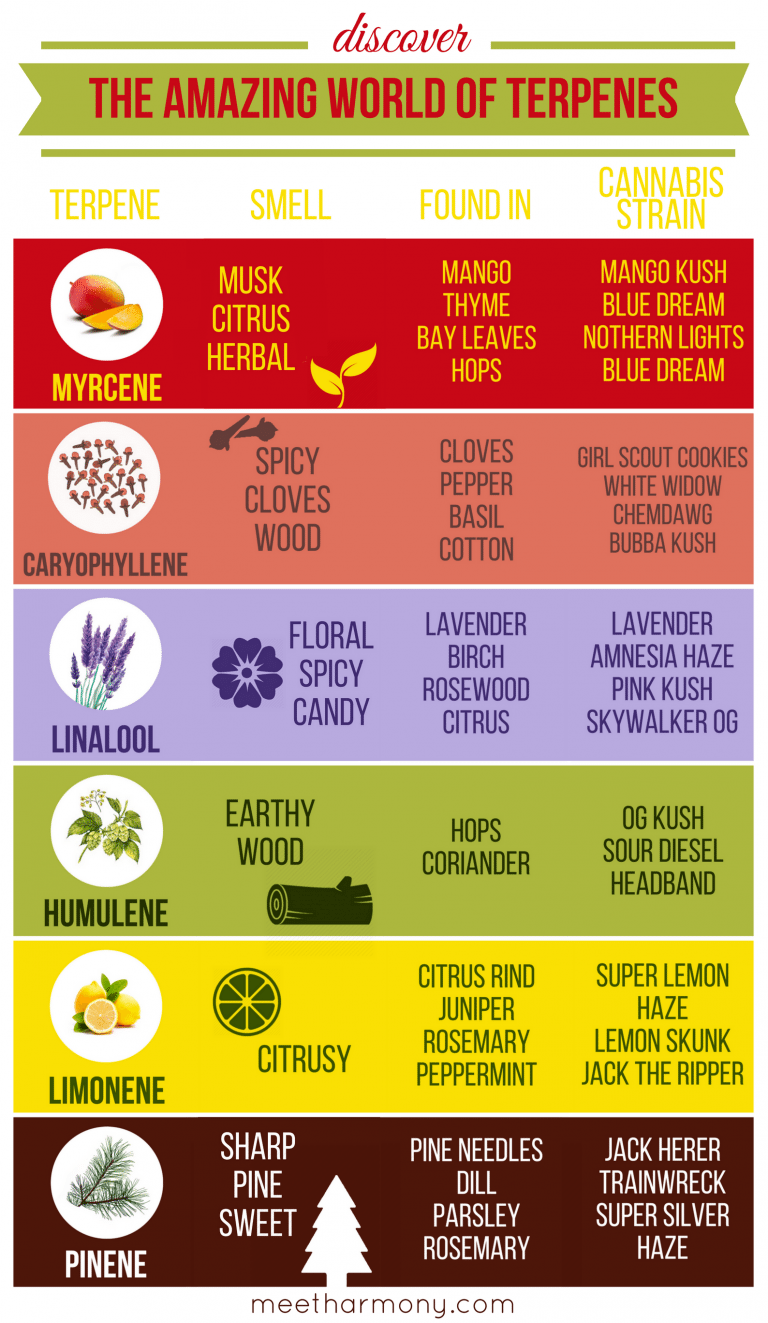
\includegraphics[width = 8.5cm]{Terpenes.png}
    \end{center}
    \caption{Base Terpenes \cite{alana2019}}
    \label{fig:baseterpenes}%
\end{figure} Terpenes mainly contribute to taste and smell factors that we perceive when consuming everything from apples and grapes to wine and cannabis, the latter of which has recently been decriminalized and has important medical and business (e.g., recreational) use cases. A desirable property of these products are brand-wise consistency; i.e., an apple of a particular brand ought to invoke a similar experience between different batches or trees, across various seasonal growing conditions, annual harvests, etc.  

Traditionally, classification of terpenes is done with a series of steps. First, the terpenes are separated by a process called gas chromatography (GC) which separates the terpenes from each other \cite{Jiang2016}. Then, the mass spectrometry will generate the mass spectrum of each separated terpene. Then the new generated mass spectrum of each terpene is detected by a chemist through library matching \cite{Jiang2016}. New generated mass spectrum of the terpenes is matched with the existing database of various samples.
%Next, the detection of the terpene is done by mass spectrometry. Mass spectrometry will generate the mass spectrum for each terpene. The undetected terpenes are detected by a chemist through library matching \cite{Jiang2016}.

The current study investigates the utility of Machine Learning (ML) algorithms as analysis tools for classifying mass spectra of synthetic cannabis samples over a variety of brands/products with the end goal of predicting the presence (or lack thereof) of specific terpene compounds and compositions. Where humans have conventionally been used in quality assurance tests (potato chip brand tests, milk spoilage, etc.), ML algorithms combined with rapid, easy-to-use and portable MS technology and devices offer the potential for more consistent, bias-free experience analysis and a multitude of improved efficiencies for producers.

\subsection{Approach Outline}
Synthetic data is generated with the help of Google Colab for all the eight terpenes with five percent resolution in each component. \\
The approach to solve the problem will be as follows:
\begin{enumerate}
  \item Generate synthetic data with all the possible combinations of the eight terpenes
  \item Labels them according to their contributions
  \item Create, train and test the model to classify the present terpenes
  \item Create, train and test the model to find the contribution of each terpene
\end{enumerate}

\subsection{Scope}

\section{Background}

\subsection{Mass Spectrometry (MS)}
A mass spectrometry is a device that vaporizes and then ionizes a sample of a compound using an electron beam. After ionization the sample fragments into radicals and cations (positively charged ions). Then, the cations will be detected by the detectors in the mass spectrometer. Mass spectrometer will generate a graph that plots the %\gls{m/z} 
m/z ratio on the x-axis and \gls{rel abund} on the y-axis. This graph is known as the mass spectrum. Every terpene has unique (x-axis, y-axis) pair values.

\begin{figure}[!ht]
\centering
    \begin{center}
        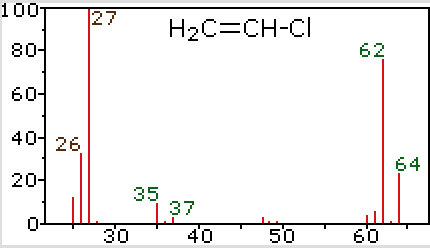
\includegraphics[width=9cm]{vyn.png}
    \end{center}
    \caption{Mass Spectrum of vinyl chloride}
    \label{fig:vyn}
\end{figure}


In the example provided in Figure \ref{fig:vyn}, 27 is the base peak which has a \gls{rel abund} of 100\%. 62 is the parent peak a.k.a. M\textsuperscript{+} or mass of a compound. For isotopes, it can be M+1 or M+2.

\subsection{Machine Learning Applications for Mass Spectrometer}
Mass spectrometer is a tool which measures mass-to-charge ratio of a compound, mixture or an isotope. Deep convolutional neural networks (CNN) are used for tumor classification. An adapted CNN architecture was designed for mass spectra, as it is different from RGB images. It classifies the imaging mass spectrometry data.

Long short-term memory (LSTM) and Convolutional Neural Networks (CNN) are integrated for peptide sequencing. To get higher accuracy, a deep learning model combining an order invariant network structure (T-net) and recurrent neural networks is designed \cite{Bhermann2017}.

\subsection{Related Work}
Intensity-based protein identification by machine learning from a library of tandem mass spectra \cite{Elias2004}.


\section{Data}
\subsection{MS data conventions}
Joint Committee on Atomic and Molecular Physical data extension (JCAMP-DX) file is the accepted standard file format in the field of chemistry to read the (x,y) coordinates to generate mass spectrum of compounds, mixtures or isotopes. JCAMP files are text files with the compound name, molecular name, owner of the data and other header information can also be added.

\subsection{Data Generation}
Synthetic data is generated for eight commonly used terpenes using an additive composition model with five percent resolution in each component. The eight base terpenes included in the current study are: myrcene, linalool, limonene, $\alpha$-pinene, $\beta$-pinene, trans-caryophyllene, cannabidiol (CBD) and tetrahydrocannabinol (THC). These terpenes are found in many food products that we consume in our day-to-day lives.  Examples are provided in fig. \ref{fig:baseterpenes} \cite{Russo2011}. Mass spectra for all possible combinations of eight terpenes sums up to 50,388. We represent these compositions as 50,388 row vectors. Let's consider first row matrix as '$M1$', shown in figure \ref{fig:dataRepresentation}. The matrix which represents y-axis (relative abundance) of a mass spectrum has 320*8 dimensions. This is denoted `$M2$' in figure \ref{fig:dataRepresentation}. M2 consists of m/z values of the eight base terpenes for all the 320 values of x-axis (m/Z values). The dot product of M1 and M2 will result in a column vector of size 320 which will be the final values of y-axis which is shown in \ref{fig:dataRepresentation}. X-axis for a mass spectrum will have m/Z values from 1-320. Each row vector (50,388 row vectors) will therefore generate 50,388 mass spectra. Labels for these combinations were generated based on the largest terpene contributor to the composition. Principal Component Analysis was performed to visualize the separation for the highest contributor terpene to the mass spectrum. %The results are shown in fig. \ref{fig:2dPCAfor8}.

\begin{figure}[!ht]
\centering
    \begin{center}
        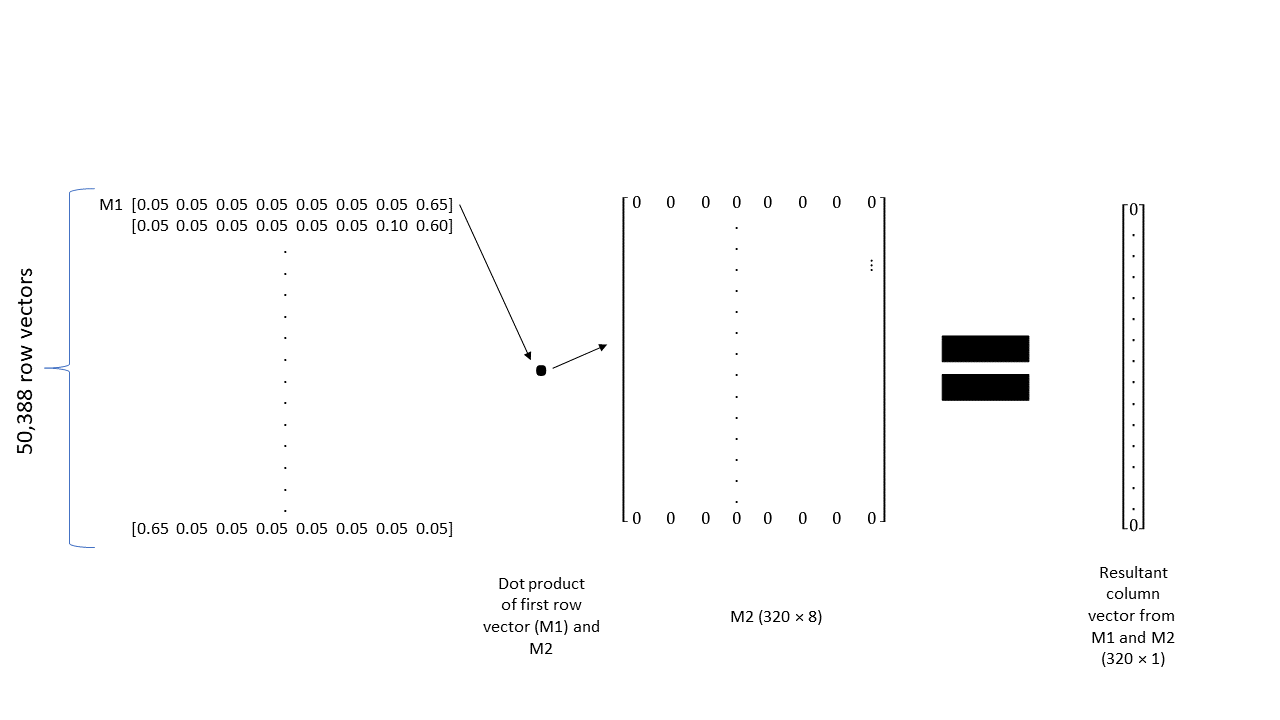
\includegraphics[width=16.2cm]{datarepresentation.png}
    \end{center}
    \caption{Calculation of resultant y-axis}
    \label{fig:dataRepresentation}
\end{figure}

The end goal is to generate a regression model that will accept a sample and output terpene compositions to ensure that the sample is consistent with the desired brand characteristics. Currently, the majority terpene contribution (in the form of a classification task) indicates that it is possible to determine what is likely to be the main flavor experienced by the consumer which can be seen in \ref{fig:confMat}, this is encouraging but more work needs to be done to decompose a sample into the baseline terpene components.

%\subsubsection{Mass Spec formats}
%\subsubsection{JCAMP}

\section{Methods}
\subsection{Approach}
In the ongoing research, a sample (consisting of multiple terpenes) is exposed to the mass spectrometer (a portable device which is developed by an industry partner company) which generates a mass spectrum. The tool that is being developed by Acadia Institute of Data Analytics will detect the terpenes present in the product and their concentration. This offers portability and automatic learning of rules that will provide a predictive decomposition from any given sample. The testing at each stage is done using four terpenes compositions to establish the key learning parameters and then tests will be run on a set of eight terpenes.

A dataset of all the possible combinations of 4 terpenes was generated for testing purposes and the plan is to switch to 8 terpenes. The total number of combinations for 4 terpenes with a resolution of 5 percent are 969. A data file is labelled with the name of terpene having the highest contribution to each combination examplar. Initial classification tests were run on WEKA (Waikato Environment for Knowledge Analysis) \cite{hall2009}. The 10-fold cross-validation method was used to test with the WEKA SVM \cite{Cortes1995} algorithm.

The end goal is to generate a regression model that will accept a sample and output terpene compositions to ensure that the sample is consistent with the desired brand characteristics. Currently, the majority terpene contribution (in the form of a classification task) indicates that it is possible to determine what is likely to be the main flavor experienced by the consumer which can be seen in \ref{fig:confMat}, this is encouraging but more work needs to be done to decompose a sample into the baseline terpene components.

\subsection{Visualization}

\subsection{\gls{PCA}}
\gls{PCA} is one of many techniques used to reduce the dimensions of inputs. The inputs are combined in a specific manner such that the least important variables can be dropped while retaining the most important variables. The simplest way to achieve the PCA algorithm is by plotting all the dimensions or variables and then finding the direction with the largest variance. \begin{figure}[!ht]
\centering
    \begin{center}
        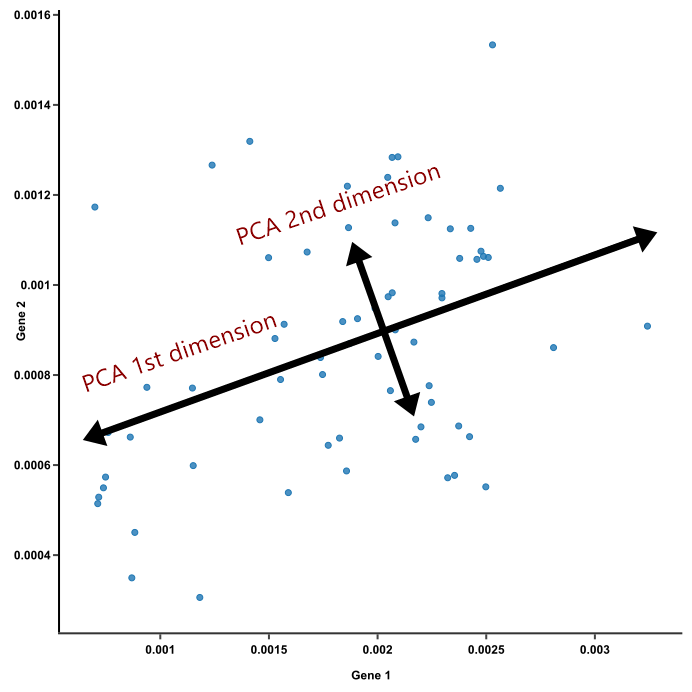
\includegraphics[width = 14.4 cm]{howPCAworks.png}
    \end{center}
    \caption{Working of PCA}
    \label{fig:howPCAWorks}
\end{figure} The orthogonal direction to the previous principal component with second largest variance can be considered as the second component. It can be seen in \ref{fig:howPCAWorks}.

The \gls{PCA} algorithm finds new sets of dimensions such that the new found dimensions are orthogonal to each other (to be linearly independent). They are ranked based on the variance of data.

The problem has 320 dimensions and 50,388 samples. It is difficult to visualise all 320 dimensions in a plot because it is difficult to draw a plot with 320 axes or dimensions. These 320 dimensions are statistically reduced to 2 dimensions which can be plotted in a 2D graph. The 50,388 samples are plotted with different colors depending on the category they belong. Grouping of these categories indicates how separable the data are. The PCA results for the project can be seen in \ref{fig:2dPCAfor8}.

\begin{figure}[!ht]
\centering
    \begin{center}
        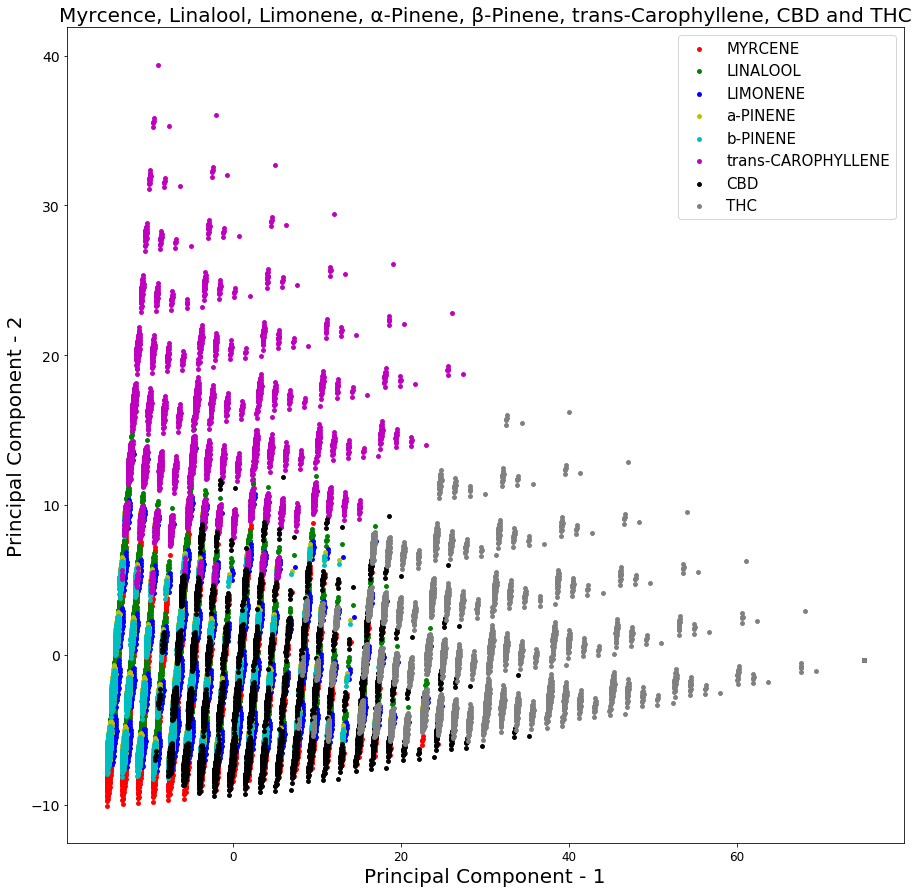
\includegraphics[width=9cm]{2dPCA.png}
    \end{center}
    \caption{Principal Component Analysis of 8 terpenes}
    \label{fig:2dPCAfor8}
\end{figure}

%\gls{PCA} reduces 320 dimensions to 2 dimensions and plots 50,388 samples to visualise how distinct these samples are. The variance of the dimensions help us to understand the performance of data in prediction. It is difficult to visualise all the 320 dimensions in a plot, because it's impossible to draw a plot with 320 axes or dimensions. So, the 320 dimensions are reduced to 2 dimensions which only shows the variance of the 320 dimensions. The final two dimensions are orthogonal to each other showing the most and the second-most variance of the data.

\section{Results}
The mean absolute error with default parameters on the dataset of 4 terpenes was 0.2581. The accuracy achieved by the SVM algorithm \cite{Cortes1995} on this dataset is 91.4345\%. In the results shown in fig. \ref{fig:confMat}.
In the confusion matrix, a, b, c, and d are myrcene, $\alpha$-pinene, THC and CBD respectively.

\begin{figure}[!ht]
\centering
    \begin{center}
        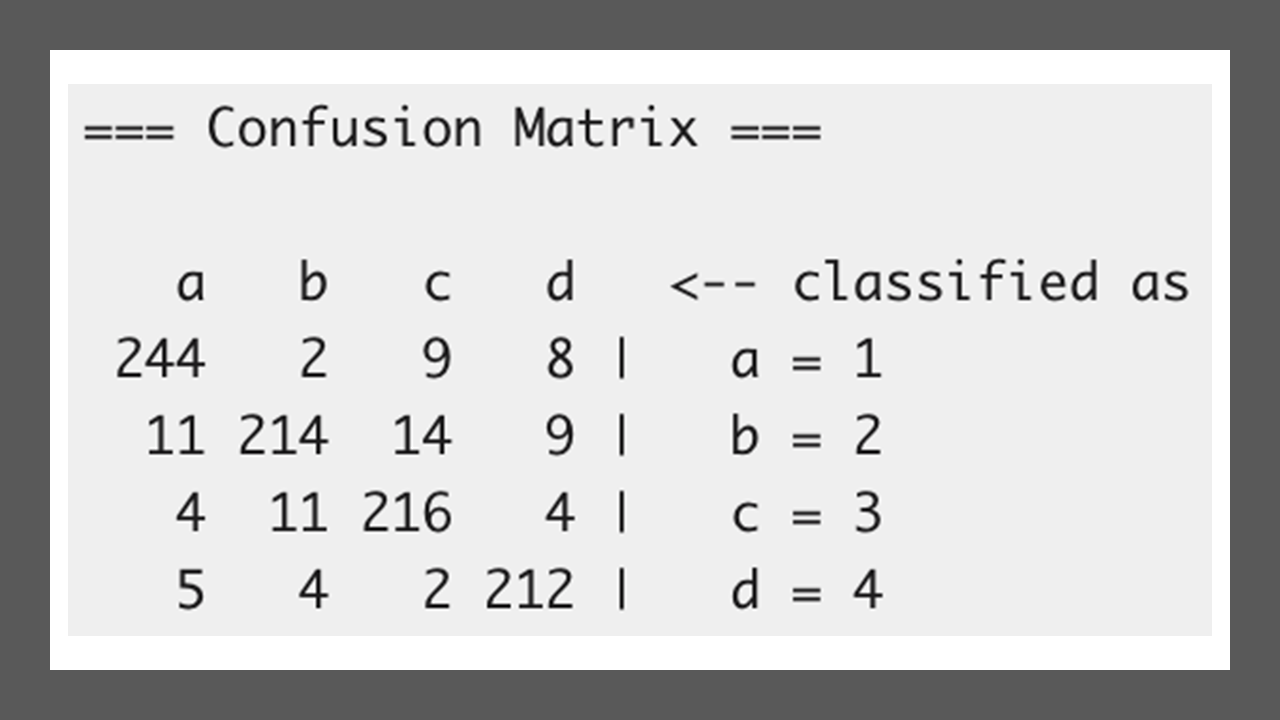
\includegraphics[width = 9 cm]{confusionMatrixforGSS2020.png}
    \end{center}
    \caption{Confusion Matrix results}
    \label{fig:confMat}
\end{figure}

\section{Conclusions}
The empirical study shows that the accuracy for 10-fold cross-validation approach is 91.43\% for the classification of four terpenes. These are the initial results which supports that the machine learning has great potential to be used in the classification of terpenes. In future work, we anticipate experimenting with deep neural networks models to compare the SVM algorithm \cite{Cortes1995} and determine the best algorithm to find the proportions of terpenes present in real-world samples.


\newpage
%\section{References}
\bibliographystyle{plain} 
\bibliography{Bibliography.bib}


%Elias, Joshua & Gibbons, Frank & King, Oliver & Roth, Frederick & Gygi, Steven. (2004). Intensity-based protein identification by machine learning from a library of tandem mass spectra. Nature biotechnology. 22. 214-9. 10.1038/nbt930. 
 
\clearpage

%\printglossary[type=\acronymtype] 



\printglossary[nonumberlist]
%\printglossary
 
\end{document}\documentclass[12pt, a4paper]{article}
\setlength{\oddsidemargin}{0.5cm}
\setlength{\evensidemargin}{0.5cm}
\setlength{\topmargin}{-1.6cm} 
\setlength{\leftmargin}{0.5cm} 
\setlength{\rightmargin}{0.5cm} 
\setlength{\textheight}{24.00cm} 
\setlength{\textwidth}{15.00cm} 

%\parindent 2pt
%\parskip 5pt
\usepackage[utf8]{inputenc}
%\usepackage{glossaries}
\usepackage[acronym]{glossaries}
\usepackage{xcolor}
\usepackage{graphicx}
\usepackage{datetime}
\usepackage{courier}
\usepackage{array}
 
\makeglossaries

\newglossaryentry{rel abund}
{
    name=relative abundance,
    description={Amount of an ion produced in comparison to the most abundant ion.}
}

\newglossaryentry{PCA}
{
    name=Principal Component Analysis,
    description={A statistical method that describes the data by inter-correlated dependant variables}
}

%\title{How to create a glossary}
%\author{ }
%\date{ }

\setlength{\parindent}{4em}
\setlength{\parskip}{1em}
\renewcommand{\baselinestretch}{1.25}
 
\begin{document}
%\maketitle

\section{Abstract}
Terpenes are an important class of organic compounds produced from fruits and vegetables that we consume every day. For instance, Myrcene is found from mango, Humulene is found from coriander. Terpenes mainly contribute to taste and smell factors that we perceive when consuming everything from apples and grapes to cannabis, which has recently been decriminalized and has important medical and business (e.g., recreational) use cases. A desirable property of these products is brand-wise consistency; i.e., an apple of a particular brand ought to invoke a similar experience between batches or trees, across various seasonal growing conditions, annual harvests, etc. The current study investigates the utility of Machine Learning (ML) algorithms as analysis tools for classifying mass spectra (MS) of cannabis samples over a variety of brands/products with the end goal of predicting the presence (or lack thereof) of specific terpene compounds and terpene compositions to pre-determine schedules for plant development, treatment routines, and market potential. Where humans have conventionally been used in quality assurance tests (potato chip brand tests, milk spoilage, etc.), ML algorithms combined with rapid, easy-to-use and portable MS technology and devices offer the potential for more consistent, bias-free experience analysis and a multitude of improved efficiencies for producers.

\section{Introduction}

\section{Background}

\subsection{Mass Spectrometry (MS)}
A mass spectrometry is a device that vaporizes and then ionizes a sample of a compound using an electron beam. After ionization the sample fragments into radicals and cations (positively charged ions). Then, the cations will be detected by the detectors in the mass spectrometer. Mass spectrometer will generate a graph that plots the %\gls{m/z} 
m/z ratio on the x-axis and \gls{rel abund} on the y-axis. This graph is known as the mass spectrum.

\begin{figure}[!ht]
\centering
    \begin{center}
        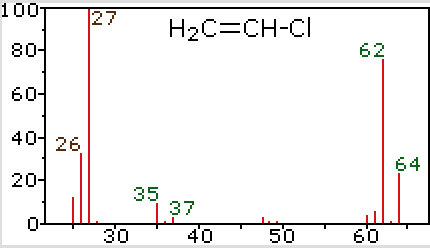
\includegraphics[width=8.5cm]{vyn.png}
    \end{center}
    \caption{Mass Spectrum of vinyl chloride}
    \label{fig:vyn}
\end{figure}


In the example provided in Figure \ref{fig:vyn}, 27 is the base peak which has a \gls{rel abund} of 100\%. 62 is the parent peak a.k.a. M\textsuperscript{+} or mass of a compound. For isotopes, it can be M+1 or M+2.

\subsection{Machine Learning Applications for Mass Spectrometer}
Mass spectrometer is a tool which measures mass-to-charge ratio of a compound, mixture or an isotope. Deep convolutional neural networks (CNN) are used for tumor classification. An adapted CNN architecture was designed for mass spectra, as it is different from RGB images. It classifies the imaging mass spectrometry data.

Long short-term memory (LSTM) and Convolutional Neural Networks (CNN) are integrated for peptide sequencing. To get higher accuracy, a deep learning model combining an order invariant network structure (T-net) and recurrent neural networks is designed \cite{Bhermann2017}.

\subsection{Related Work}
Intensity-based protein identification by machine learning from a library of tandem mass spectra \cite{Elias2004}.


\section{Data}
\subsection{MS data conventions}
Joint Committee on Atomic and Molecular Physical data extension (JCAMP-DX) file is the accepted standard file format in the field of chemistry to read the (x,y) coordinates to generate mass spectrum of compounds, mixtures or isotopes. JCAMP files are text files with the compound name, molecular name, owner of the data and other header information can also be added. 

%\subsubsection{Mass Spec formats}
%\subsubsection{JCAMP}

\section{Methods}
\subsection{Visualization}


\subsection{\gls{PCA}}
\gls{PCA} is one of many techniques used to reduce the dimensions of inputs. The inputs are combined in a specific manner such that the least important variables can be dropped while retaining the most important variables. The simplest way to achieve the PCA algorithm is by plotting all the dimensions or variables and then finding the direction with the largest variance. The orthogonal direction to the previous principal component with second largest variance can be considered as the second component. More variance shows more information.

The \gls{PCA} algorithm finds new sets of dimensions such that the new found dimensions are orthogonal to each other (to be linearly independent). They are ranked based on the variance of data.

The problem has 320 dimensions and 50,388 samples. It is difficult to visualise all 320 dimensions in a plot because it is difficult to draw a plot with 320 axes or dimensions. These 320 dimensions are statistically reduced to 2 dimensions which can be plotted in a 2D graph. The 50,388 samples are plotted with different colors depending on the category they belong. Grouping of these categories indicates how separable the data are.

%\gls{PCA} reduces 320 dimensions to 2 dimensions and plots 50,388 samples to visualise how distinct these samples are. The variance of the dimensions help us to understand the performance of data in prediction. It is difficult to visualise all the 320 dimensions in a plot, because it's impossible to draw a plot with 320 axes or dimensions. So, the 320 dimensions are reduced to 2 dimensions which only shows the variance of the 320 dimensions. The final two dimensions are orthogonal to each other showing the most and the second-most variance of the data.

\section{Results}

\section{Conclusions}

\newpage
%\section{References}
\bibliographystyle{plain} 
\bibliography{Bibliography.bib}


%Elias, Joshua & Gibbons, Frank & King, Oliver & Roth, Frederick & Gygi, Steven. (2004). Intensity-based protein identification by machine learning from a library of tandem mass spectra. Nature biotechnology. 22. 214-9. 10.1038/nbt930. 
 
\clearpage

%\printglossary[type=\acronymtype] 



\printglossary[nonumberlist]
%\printglossary
 
\end{document}